\chapter{数组}\label{fortran_array}

迄今为止我们折腾的东东都是标量 (scalar), 那都是小 case, 大 case 是数组 (array). 数组的名字虽然是 ``数'' 组, 但其实数组可以是任意类型的, 只不过平常俺们用的数组基本上都是数字型的, 俺就只讲数字型的了. 数组这个东东, 俺觉得俺讲起来和初学编程的同学们理解起来都会是十分困难滴, 对俺来说, 彻底讲清楚数组最好的办法就是来一大堆数学定义, 但偏偏绝大部分同学都一看数学定义就头大, 俺只能不管了. 另外, 之前俺们讲代码的时候, 实际上经常使用左右中括号 \ttt{[]}, 表示左右中括号和里头的内容需要按需求被替换, 但笔记写到这里俺突然发现左右中括号从本章开始有大用, 所以从本章开始俺们会改使用左右大括号 \ttt{\{\}}, 表示左右大括号和里头的内容需要按需求被替换.

\section{数组基础}\label{fortran_array_basic}

Fortran 中的数组分为全数组 (whole array) 和非全数组, 先讲全数组.
全数组是一个映射 $
    a\colon  S_1 \times \dots \times S_n \to \mathbb{C},\,
        (s_1, \dots, s_n) \mapsto a_{s_1\dots s_n}
$, 其中任意 $i \in \{1, \dots, n\}$, $S_i = \{j_i, \dots, k_i\} \subset \mathbb{Z}$. 换言之, 全数组是一堆带着 $n$ 个整数下标的复数 $a_{s_1\dots s_n}$, $s_1, \dots, s_n$ 的取值范围分别是 $\{j_1, \dots, k_1\}, \dots, \{j_n, \dots, k_n\}$. 数组的应用非常多, 数学中的向量, 矩阵\footnote{同学们会学到的.}, 物理中的矢量, 张量\footnote{同学们会学到的.}都可以表示成数组, 所以这一章特别是这一节同学们铁定得啃下来呢.

按上一段中数组的映射定义, 定义一个数组 $a$, 则定义中的正整数 $n$ 称为数组 $a$ 的维数/秩 (rank), 标量相当于 $0$ 维数组. 任意 $i \in \{1, \dots, n\}$, 称数组 $a$ 有第 $i$ 个维度 (dimension), 整数 $j_i$ 和整数 $k_i$ 分别称为数组 $a$ 的第 $i$ 个维度的下界 (lower-bound) 和上界 (upper-bound), $\{j_i, \dots, k_i\}$ 的元素个数 $l_i=(k_i-j_i)+1$ 称为数组 $a$ 的第 $i$ 个维度的长度 (extent). 向量 $(l_1, \dots, l_n)$ 称为数组 $a$ 的形状(shape), 其本身被认定成 $1$ 维数组, 正整数 $l_1\times\dots\times l_n$ 称为数组 $a$ 的大小 (size). 数组 $a$ 的值域中的任意元素 $a_{s_1\dots s_n}$ 称为数组 $a$ 的一个元素 (element), $s_1, \dots, s_n$ 中的第 $i$ 个整数 $s_i$ 称为 $a_{s_1\dots s_n}$ 的第 $i$ 个下标/索引 (subscript/index). 以上这一大堆定义是同学们需要牢记的.

若程序中变量 \ttt{a} 代表全数组 $a$, 则 \ttt{rank(a)}, \ttt{lbound(a)}, \ttt{ubound(a)}, \ttt{shape(a)}, \ttt{size(a)} 分别是全数组 $a$ 的维数 $n$, 由所有维度的下界组成的向量 $(j_1, \dots, j_n)$, 由所有维度的上界组成的向量 $(k_1, \dots, k_n)$, 形状$(l_1, \dots, l_n)$, 大小 $l_1\times\dots\times l_n$.

同学们玩数组的时候的难点通常是不能领会数据结构 (data structure), 而数据结构正是程序设计的灵魂. 最简单帮助同学们领会数据结构的方式就是让数据结构直观化. 例如一个 $1$ 维数组 $a\colon \{1,2,3\}\to\mathbb{C}$, 我们可以把它想象成一横条 $[a_1\,a_2\,a_3]$, 但数学中通常喜欢把这横条竖起来摆. 又例如一个 $2$ 维数组 $a\colon \{1,2,3\}\times\{1,2,3\}\to\mathbb{C}$, 我们可以把它想象成一大方表
\begin{equation*}
    \begin{bmatrix}
        a_{11}&a_{12}&a_{13}\\
        a_{21}&a_{22}&a_{23}\\
        a_{31}&a_{32}&a_{33}
    \end{bmatrix}.
\end{equation*}
$3$ 维数组就麻烦了, 我们需要想象有一大堆正方体小箱子堆成一个大长方体, 每个小箱子中都装着一个复数. 更高维的数组就更麻烦了, 例如 $4$ 维数组, 只能要么想象成有一大堆正方体小箱子堆成一个 `` $4$ 维大长方体'', 每个小箱子中都装着一个复数, 要么想象成一横条, 横条由大长方体排列成, 每个大长方体都由一大堆正方体小箱子堆成, 每个小箱子中都装着一个复数.

\def\la{\leftarrow}
\def\ra{\rightarrow}
\def\ua{\uparrow}
\def\da{\downarrow}
Fortran 数组中的元素有一个被规定死的排列顺序: 任意 $a_{s_1\dots s_n}$ 和 $a_{t_1\dots t_n}$, 当 $s_{i+1}=t_{i+1}, \dots, s_n=t_n$ 时, 若 $s_i<t_i$, 则 $a_{s_1\dots s_n}$ 在 $a_{t_1\dots t_n}$前面, 若 $s_i>t_i$, 则 $a_{s_1\dots s_n}$ 在 $a_{t_1\dots t_n}$ 后. 如果用 \ttt{print *,} 输出数组, 那么 Fortran 会按元素顺序挨个输出数组中的每个元素. Fortran 规定的排列顺序称为列优先顺序 (column-major order). Matlab 学 Fortran, 也是列优先顺序. C 规定的排列顺序不一样, 是行优先顺序 (row-major order), Python 学 C, 也是行优先顺序. 例如一个 $2$ 维数组 $a\colon \{1,2\}\times\{1,2\}\to\mathbb{C}$, 在 Fortran 规定的列优先顺序中, 位置最前的下标变动最快, 排序是 $a_{11},a_{21},a_{12},a_{22}$, 如图 \ref{column_major} 所示, 在 C 规定的行优先顺序中, 位置最后的下标变动最快, 排序是 $a_{11},a_{12},a_{21},a_{22}$, 如图 \ref{row_major} 所示.
\begin{figure}[htbp]
    \centering
    \begin{tikzpicture}
        \node [circle] (a11) at (-1,1) {$a_{11}$};
        \node [circle] (a12) at (1,1) {$a_{12}$};
        \node [circle] (a21) at (-1,-1) {$a_{21}$};
        \node [circle] (a22) at (1,-1) {$a_{22}$};
        \draw [->] (a11.south) --  (a21.north);
        \draw [->] (a21.north east) --  (a12.south west);
        \draw [->] (a12.south) --  (a22.north);
    \end{tikzpicture}
    \caption{Fortran 规定的列优先顺序示意图}
    \label{column_major}
\end{figure}
\begin{figure}[htbp]
    \centering
    \begin{tikzpicture}
        \node [circle] (a11) at (-1,1) {$a_{11}$};
        \node [circle] (a12) at (1,1) {$a_{12}$};
        \node [circle] (a21) at (-1,-1) {$a_{21}$};
        \node [circle] (a22) at (1,-1) {$a_{22}$};
        \draw [->] (a11.east) --  (a12.west);
        \draw [->] (a12.south west) --  (a21.north east);
        \draw [->] (a21.east) --  (a22.west);
    \end{tikzpicture}
    \caption{C 规定的行优先顺序示意图}
    \label{row_major}
\end{figure}

如果两个数组 $a$ 和 $b$, 它们的形状一样, 那么这两个数组的元素有自然的一一对应关系, 即按 Fortran 规定的元素排列顺序, $a$ 的元素中排在第 $i$ 个的元素和 $b$ 的元素中排在第 $i$ 个的元素是对应的. 换言之, 如果用相同的直观化方法来展示 $a$ 和 $b$ 的元素, 那么 $a$ 和 $b$ 的元素中摆在相同位置的元素是对应的. 例如一个 $2$ 维数组 $a\colon \{0,1,2\}\times\{0,1\}\to\mathbb{C}$ 和另一个 $2$ 维数组 $b\colon \{1,2,3\}\times\{1,2\}\to\mathbb{C}$, 它们的元素对应关系如图 \ref{element_corresponding} 所示.
\begin{figure}[htbp]
    \centering
    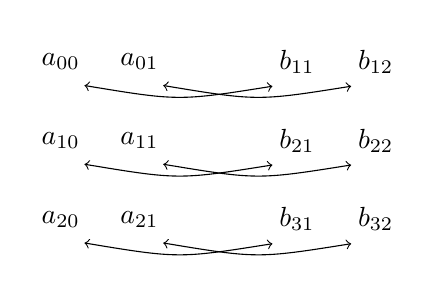
\begin{tikzpicture}
        \node [circle] (a00) at (-2,1) {$a_{00}$};
        \node [circle] (a01) at (-1,1) {$a_{01}$};
        \node [circle] (a10) at (-2,0) {$a_{10}$};
        \node [circle] (a11) at (-1,0) {$a_{11}$};
        \node [circle] (a20) at (-2,-1) {$a_{20}$};
        \node [circle] (a21) at (-1,-1) {$a_{21}$};
        \node [circle] (b11) at (1,1) {$b_{11}$};
        \node [circle] (b12) at (2,1) {$b_{12}$};
        \node [circle] (b21) at (1,0) {$b_{21}$};
        \node [circle] (b22) at (2,0) {$b_{22}$};
        \node [circle] (b31) at (1,-1) {$b_{31}$};
        \node [circle] (b32) at (2,-1) {$b_{32}$};
        \draw [<->] (a00.south east) .. controls (-0.5,0.5) .. (b11.south west);
        \draw [<->] (a01.south east) .. controls (0.5,0.5) .. (b12.south west);
        \draw [<->] (a10.south east) .. controls (-0.5,-0.5) .. (b21.south west);
        \draw [<->] (a11.south east) .. controls (0.5,-0.5) .. (b22.south west);
        \draw [<->] (a20.south east) .. controls (-0.5,-1.5) .. (b31.south west);
        \draw [<->] (a21.south east) .. controls (0.5,-1.5) .. (b32.south west);
    \end{tikzpicture}
    \caption{元素对应关系示意图}
    \label{element_corresponding}
\end{figure}

如果两个数组可以有元素对应关系, 那么它们需要有相同的形状, 但它们的每个维度都不需要有相同的上下界. 非全数组是和全数组一样具有确定的形状, 但每个维度都没有确定的上下界的数组, 也就是说, 非全数组和全数组一样可以用横条, 方表等进行直观化表示, 可以和全数组有元素对应关系, 但非全数组中的元素都无法写出其下标. 若程序中变量 \ttt{a} 代表非全数组 $a$, 则 \ttt{rank(a)}, \ttt{shape(a)}, \ttt{size(a)} 仍然分别是非全数组 $a$ 的维数 $n$, 形状$(l_1, \dots, l_n)$, 大小 $l_1\times\dots\times l_n$, 而 \ttt{lbound(a)}, \ttt{ubound(a)} 则分别是由 $n$ 个 $1$ 组成的向量 $(1, \dots, 1)$, 由所有维度的长度组成的向量 $(l_1, \dots, l_n)$, 仿佛每个维度的下界都确定是 $1$ 一样 (但其实不是). 为表述方便, 以下会用形状和非全数组相同的, 每个维度的下界都确定是 $1$ 的全数组来表示非全数组.

\section{数组构造}\label{fortran_array_construction}

我们可以用数组构造器 (array constructor) 来构造\uline{一维}数组常量. 用数组构造器构造出来的一维数组常量都是非全数组. 数组构造器的用法复杂至极, 我们只学两种用法. 所有数组构造器都形如 \ttt{[...]}, 且两边的 \ttt{[} 和 \ttt{]} 都可以用 \ttt{(/} 和 \ttt{/)} 替代而写成 \ttt{(/.../)}.

第一种用法是直接写 \ttt{[a1, ..., an]}, \ttt{a1, ..., an} 中的任意 \ttt{ai} 是值为 $a_i$ 的标量, 来代表 $[a_1, ..., a_n]$. 例如 \ttt{[1, 2, 3]} 代表 $[1, 2, 3]$, 非常简单.

第二种用法是用隐式 do 循环 (implied DO loop), 这玩意儿比较难. 同学们需要掌握常用的一重隐式 do 循环, 如果老师敢考难死人的多重隐式 do 循环, 俺们就赶紧揭竿而起\dots{} 假如我们要造个数组 $[1, \dots, 1000]$, 写 \ttt{[1, ..., 1000]} 肯定不成, 这时我们可以写 \ttt{[(i, i = 1, 1000)]}, 其中 \ttt{i} 必须是\uline{声明过的}整型变量. 一般地, 隐式 do 循环 \ttt{[(\{expr\}, \{m\} = \{m1\}, \{m2\}, \{m3\})]} 的第 $i$ 个元素是下面这样的显式 do 循环输出的第 $i$ 个数, 其中 \ttt{, \{m3\}} 若省略, \ttt{\{m3\}} 则为 \ttt{1}.
\begin{lstlisting}[numbers=none]
do {m} = {m1}, {m2}, {m3}
    print *, {expr}
end do
\end{lstlisting}
例如 \ttt{[(n**2, n = 1, 10, 2)]} 代表 $[1^2, 3^2, 5^2, 7^2, 9^2]$. 再次提醒, \ttt{\{m\}} 必须是\uline{声明过的}整型变量.

Ifx 有器规, 可以用简写 \ttt{[\{m1\}:\{m2\}:\{m3\}]} 代替 \ttt{[(\{m\}, \{m\} = \{m1\}, \{m2\}, \{m3\})]}. 这种不规范的写法同学们不许用.

一般地, 多重隐式 do 循环 \ttt{[(...(\{expr\}, {m\_{}1} = \{m1\_{}1\}, \{m2\_{}1\}, \{m3\_{}1\}), ..., {m\_{}n} = \{m1\_{}n\}, \{m2\_{}n\}, \{m3\_{}n\})]} 的第 $i$ 个元素是下面这样的多重显式 do 循环输出的第 $i$ 个数, 其中 \ttt{, \{m3\_{}i\}} 若省略, \ttt{\{m3\_{}i\}} 则为 \ttt{1}.
\begin{lstlisting}[numbers=none]
do {m_n} = {m1_n}, {m2_n}, {m3_n}
    ......
        do {m_1} = {m1_1}, {m2_1}, {m3_1}
            print *, expr
        end do
    ......
end do
\end{lstlisting}
例如 \ttt{[((m+n**2, m = 0, 1), n = 1, 2)]} 代表 $[0+1^2, 1+1^2, 0+2^2, 1+2^2]$. Python 有一个和多重隐式 do 循环很相似的, 叫列表推导式的东东, 能给出多维数组. 但请注意, Fortran 的多重隐式 do 循环只能给出\uline{一维}数组常量, 如果需要多维数组常量, 那么需要用 \ref{fortran_array_manipulation} 节讲的数组操作把一维数组常量变成多维数组常量.

\section{数组声明}\label{fortran_array_specification}

用数组变量和数组具名常量之前当然要声明. 在数组声明中需要声明数组的类型, 还可以另外声明数组的种别, 数组的类型/种别是数组中的每个元素的类型/种别.

在数组声明中还需要给数组加上 dimension 属性, 来确定数组的维数和每个维度的上下界\footnote{这表明数组变量和数组具名常量是全数组.}. 有两种方法可行, 一种是直接在声明的 \ttt{::} 后面的数组变量/数组具名常量的名称的后面加 \ttt{(j1:k1, ..., jn:kn)}, 一种是在声明的 \ttt{::} 前面加 \ttt{, dimension(j1:k1, ..., jn:kn)}. \ttt{j1}, \dots, \ttt{jn} 中的所有 \ttt{ji} 和 \ttt{k1}, \dots, \ttt{kn} 中的所有 \ttt{ki} 都必须是整型常量 (或整型常量表达式). \ttt{j1:k1}, \dots, \ttt{jn:kn} 中的所有 \ttt{ji:} 都可省略, 若省略, 则 \ttt{ji} 为 \ttt{1}, 换言之, Fortran 数组的任意维度的下界默认是 \ttt{1}. Matlab 学 Fortran, 也默认是 \ttt{1}. C 不一样, 默认是 \ttt{0}, Python 学 C, 也默认是 \ttt{0}. 下面是数组声明示例.
\begin{lstlisting}
program main
    implicit none
    real :: array1(10, 10)
    real, dimension(10, 10) :: array2
    real :: array3(1:10, 1:10)
    real, dimension(1:10, 1:10) :: array4
end program main
\end{lstlisting}
选择哪种声明方式呢? 一般大家喜欢用不写 \ttt{dimension} 的第一种方式, 毕竟少打几个字, 而且看着比较简洁. 但如果是要一口气声明一堆上下界都一样的数组, 这时第一种方式反而不好使了, 大家就喜欢用写 \ttt{dimension} 的第二种方式. 下面也是数组声明示例.
\begin{lstlisting}
program main
    implicit none
    real :: a(1, 1), b(2, 2), c(3, 3)
    real, dimension(4, 4) :: d, e, f
end program main
\end{lstlisting}

如果是声明数组具名常量, 那么我们可以在声明时把任意维度的上界写成 \ttt{*}, 这样数组具名常量的这个维度的上界直接由初始化时使用的数组字面常量确定, 非常方便. 不过这种数组的名字和字符串不一样, 不叫假定形状数组 (假定形状数组在 \ref{assumed-shape} 小节讲), 而叫隐式形状数组 (implied-shape array). 下面是隐式形状数组示例, 其中数组具名常量 \ttt{v} 唯一的维度的下界为 \ttt{1} (声明中 \ttt{*} 前的 \ttt{1:} 可省略), 上界为 \ttt{3}.
\begin{lstlisting}
program main
    implicit none
    real, parameter :: v(1:*) = [0.1, 1.1, 2.1]
end program main
\end{lstlisting}

和延迟长度字符串类似, 我们可以在声明中除去所有 \ttt{ji:ki} 中的 \ttt{ji} 和 \ttt{ki}, 剩下 \ttt{:}, 并附带地用 \ttt{allocatable} 加上 allocatable 属性, 来表示声明的是延迟形状数组 (deferred-shape array). 延迟形状数组各维度的上下界在声明后未定, 但维数确定. 任意延迟形状数组 \ttt{a}, 我们可以用形如 \ttt{allocate(a(j1:k1, ..., jn:kn))} 的 allocate 语句让 \ttt{a} 各维度的下界确定成 \ttt{j1}, \dots, \ttt{jn} (任意 \ttt{j1:} 仍可省略), 上界确定成 \ttt{k1}, \dots, \ttt{kn}, 用形如 \ttt{deallocate(a)} 的 deallocate 语句让 \ttt{a} 各维度的上下界未定. 这也意味着延迟形状数组只能是变量. 示例如下.
\begin{lstlisting}
program main
    implicit none
    real, allocatable :: array1(:)
    real, dimension(:, :), allocatable :: array2
    allocate(array1(10))
    allocate(array2(10, 10))
    deallocate(array1)
    deallocate(array2)
end program main
\end{lstlisting}
请注意使用 allocate 语句的时候数组的维数要匹配. 例如下面这个例子, \ttt{a} 是二维的, 但 allocate 语句却想让 \ttt{a} 是一维的, 这将失败.
\begin{lstlisting}
program main
    implicit none    
    real, allocatable :: a(:, :)
    allocate(a(10)) ! Error: ranks are different!
end program main
\end{lstlisting}

和延迟长度字符串类似, \ref{fortran_array_assignment} 节将介绍, 我们给延迟形状数组赋值的时候, 电脑会自动使用 allocate 语句和 deallocate 语句, 我们不用操心了. 但是, 如果程序运行到某时已经不需要使用某个延迟形状数组, 请对那个延迟形状数组使用 deallocate 语句. 需要这么做的原因是, 通常情况下如果程序运行到某时已经不需要使用某个变量, 那个变量很可能会被电脑自动删掉, 这个操作的学名是垃圾回收 (garbage collection), 但因为延迟形状数组需要我们或电脑手动用 allocate 语句和 deallocate 语句操作一番, 所以延迟形状数组很可能不会被电脑自动删掉, 偏偏实践中的延迟形状数组又通常巨大无比, 1 个 G 都完全不算什么, 最后的结果是大大的延迟形状数组一直把内存占着, 电脑不堪重负, 程序跑得慢甚至崩溃出错. 所以我们得老老实实不厌其烦地用 deallocate 语句, 它能让延迟形状数组把内存让出来. 延迟长度字符串本也有这个问题, 但实践中的延迟长度字符串通常很小 (天文人经常做大规模数据处理, 但不经常做大规模文本处理), 这个问题姑且可以无视.
\begin{convention}
    如果程序运行到某时已经不需要使用某个有 allocatable 属性的变量, 那么对这个变量使用 deallocate 语句.
\end{convention}

\section{数组操作}\label{fortran_array_manipulation}

我们可以对数组进行变形 (reshape), 这很简单. 变形就是用一个旧数组来造一个形状未必一样的新数组, 使得新数组中排在第 $i$ 个的元素和旧数组中排在第 $i$ 个的元素相同, 换言之, 把旧数组中的元素按元素顺序复制出来, 再按元素顺序重新排列成某种形状来生成新数组. 如果 \ttt{\{a\}} 是旧数组, 那么 \ttt{reshape(\{a\}, \{shape\})} (其中 \ttt{\{shape\}} 是一维数组) 是对旧数组 \ttt{\{a\}} 进行变形得到的形状为 \ttt{\{shape\}} 的新数组. 例如, 假设我们想造式 \eqref{a1} 中的数组,
\begin{equation}
    \begin{bmatrix}
        1&4&7\\
        2&5&8\\
        3&6&9
    \end{bmatrix}\label{a1}
\end{equation}
我们可以把 \ttt{[(i, i = 1, 9)]} 变形成形状为 \ttt{[3, 3]} 的数组, 因此我们写 \ttt{reshape([(i, i = 1, 9)], [3, 3])} 即可.

我们可以对数组进行转置 (transpose), 这有点儿难. 用数学来说, 设旧数组可表示为 $a_{s_1\dots s_n}$, 新数组可表示为 $b_{s_1\dots s_n}$, 另给表示 $a_{s_1\dots s_n}$ 和 $b_{s_1\dots s_n}$ 的维度的关系的\uline{一维整型}向量, 用 \ttt{\{order\}} 表示, 此向量中的元素按顺序依次为 $i_1$, \dots{}, $i_n$, 则 $b_{s_1\dots s_n}=a_{s_{i_1}\dots s_{i_n}}$. 直观化地理解, 请同学们想象有一个 $n$ 维空间, 坐标轴为 $s_1$ 轴, \dots{} $s_n$ 轴, 数组 $a$ 的元素 $a_{s_1\dots s_n}$ 挂在坐标点 $(s_1, \dots, s_n)$ 上, 然后我们变换空间的坐标轴, 让旧 $s_1$ 轴变成新 $s_{i_1}$ , \dots{} 旧 $s_n$ 轴变成新 $s_{i_n}$, 变换后挂在坐标点 $(s_1, \dots, s_n)$ 上的元素就是 $b$ 的元素 $b_{s_1\dots s_n}=a_{s_{i_1}\dots s_{i_n}}$. 我们需要更具体的例子. 假设我们想把式 \eqref{a1} 中的数组转置成式 \eqref{a2} 中的数组.
\begin{equation}
    \begin{bmatrix}
        1&2&3\\
        4&5&6\\
        7&8&9
    \end{bmatrix}\label{a2}
\end{equation}
我们先给式 \eqref{a1} 中的数组补上坐标轴如图 \ref{a1_} 所示,
\begin{figure}[htbp]
    \centering
    \begin{tikzpicture}
        \node [circle] (p1) at (-1,1) {$1$};
        \node [circle] (p2) at (-1,0) {$2$};
        \node [circle] (p3) at (-1,-1) {$3$};
        \node [circle] (p4) at (0,1) {$4$};
        \node [circle] (p5) at (0,0) {$5$};
        \node [circle] (p6) at (0,-1) {$6$};
        \node [circle] (p7) at (1,1) {$7$};
        \node [circle] (p8) at (1,0) {$8$};
        \node [circle] (p9) at (1,-1) {$9$}; 
        \draw [->] (-1.5,1.5) -- (1.5,1.5);
        \draw [->] (-1.5,1.5) -- (-1.5,-1.5);
        \node [circle] (s1) at (-1.5,-2) {$s_1$};
        \node [circle] (s2) at (2,1.5) {$s_2$};
    \end{tikzpicture}
    \caption{式 \eqref{a1} 中的数组补坐标轴后所得图}
    \label{a1_}
\end{figure}
再给式 \eqref{a2} 中的数组补上坐标轴如图 \ref{a2_} 所示,
\begin{figure}[htbp]
    \centering
    \begin{tikzpicture}
        \node [circle] (p1) at (-1,1) {$1$};
        \node [circle] (p2) at (0,1) {$2$};
        \node [circle] (p3) at (1,1) {$3$};
        \node [circle] (p4) at (-1,0) {$4$};
        \node [circle] (p5) at (0,0) {$5$};
        \node [circle] (p6) at (1,0) {$6$};
        \node [circle] (p7) at (-1,-1) {$7$};
        \node [circle] (p8) at (0,-1) {$8$};
        \node [circle] (p9) at (1,-1) {$9$}; 
        \draw [->] (-1.5,1.5) -- (1.5,1.5);
        \draw [->] (-1.5,1.5) -- (-1.5,-1.5);
        \node [circle] (s1) at (-1.5,-2) {$s_1$};
        \node [circle] (s2) at (2,1.5) {$s_2$};
    \end{tikzpicture}
    \caption{式 \eqref{a2} 中的数组补坐标轴后所得图}
    \label{a2_}
\end{figure}
对比图 \ref{a1_} 和图 \ref{a2_}, 我们可发现旧 $s_1$ 轴是新 $s_2$ 轴, 旧 $s_2$ 轴是新 $s_1$ 轴, 所以表示维度的关系的向量 \ttt{\{order\}} 应是 \ttt{[2, 1]}. 如果 \ttt{\{a\}} 是旧数组, 那么 \ttt{reshape(\{a\}, shape(\{a\}), order=\{order\})} 是转置后的新数组. 因此我们写 \ttt{reshape(reshape([(i, i = 1, 9)], [3, 3]), shape(reshape([(i, i = 1, 9)], [3, 3])), order=[2, 1])} 即可.

请同学们练熟数组的变形和转置, 然后我们学简化的语法. 在上一段的示例中, 我们干了两步, 先变形后转置, 代码写得老长. 我们可以直接把 \ttt{reshape(reshape(\{a\}, \{shape\}), shape(\{a\}), order=\{order\})} 简写成 \ttt{reshape(\{a\}, \{shape\}, order=\{order\})}, 所以我们可以写 \ttt{reshape ([(i, i = 1, 9)], [3, 3], order=[2, 1])}.

我们可以对数组进行取元, 得到数组中的元素, 这超简单. 设 \ttt{a} 为数组 $a$, 而 \ttt{s1, ..., sn} 为整数 $s_1, \dots, s_n$, 则 \ttt{a(s1, ..., sn)} 为 $a_{s_1\dots s_n}$, 例如 \ttt{a(1, 3)} 是 $a_{13}$.

我们可以获取数组片段 (section), 这难上天了. 我先来讲用向量下标 (vector subscript) 来获取数组片段, 但即使是 Python 那里, 向量下标也是超级难点, 如果老师敢考难死人的向量下标, 俺们就赶紧揭竿而起\dots{} 首先我们需要数组 \ttt{a}, 表示 $a_{s_1\dots s_n}$. 然后我们需要 $n$ 个\uline{一维整型}向量 \ttt{i1, ..., in}, 分别表示 $[{i_1}_1, \dots, {i_1}_{l_1}], \dots, [{i_n}_1, \dots, {i_n}_{l_n}]$, 那么 \ttt{a(i1, ..., in)} 的元素可一一对应于形状为 $[l_1, \dots, l_n]$ 的数组 $b_{s_1\dots s_n}$ 的元素, 并且 $b_{ s_1\dots s_n }=a_{ {i_1}_{s_1}\dots {i_n}_{s_n} }$. 请看下面这个例子.
\begin{lstlisting}
program main
    implicit none
    integer :: i, a(3, 3)
    a = reshape([(i, i = 1, 9)], [3, 3])
    print *, a([1, 3, 2], [2, 1, 1, 3])
end program main
\end{lstlisting}
这个例子中 \ttt{a} 的元素可以排成表, 如 \eqref{a_whole} 所示.
\begin{equation}
    \begin{bmatrix}
        a_{11}&a_{12}&a_{13}\\
        a_{21}&a_{22}&a_{23}\\
        a_{31}&a_{32}&a_{33}
    \end{bmatrix}\label{a_whole}
\end{equation}
先可确定例子中的数组片段形状为 $[3, 4]$, 我们先在一个 $3\times4$ 的表中填满 $a_{??}$, 并在周围补上坐标轴, 如图 \ref{a_section_step_1} 所示.
\begin{figure}[htbp]
    \centering
    \begin{tikzpicture}
        \node [circle] (a11) at (-1.5,1) {$a_{??}$};
        \node [circle] (a12) at (-0.5,1) {$a_{??}$};
        \node [circle] (a13) at (0.5,1) {$a_{??}$};
        \node [circle] (a14) at (1.5,1) {$a_{??}$};
        \node [circle] (a21) at (-1.5,0) {$a_{??}$};
        \node [circle] (a22) at (-0.5,0) {$a_{??}$};
        \node [circle] (a23) at (0.5,0) {$a_{??}$};
        \node [circle] (a24) at (1.5,0) {$a_{??}$};
        \node [circle] (a31) at (-1.5,-1) {$a_{??}$};
        \node [circle] (a32) at (-0.5,-1) {$a_{??}$};
        \node [circle] (a33) at (0.5,-1) {$a_{??}$};
        \node [circle] (a34) at (1.5,-1) {$a_{??}$};
        \draw [->] (-2,1.5) -- (2,1.5);
        \draw [->] (-2,1.5) -- (-2,-1.5);
        \node [circle] (s1) at (-2,-2) {$s_1$};
        \node [circle] (s2) at (2.5,1.5) {$s_2$};
    \end{tikzpicture}
    \caption{填满 $a_{??}$ 并在周围补上坐标轴后所得图}
    \label{a_section_step_1}
\end{figure}
向量 \ttt{i1} 是 $[1, 3, 2]$, 向量 \ttt{i2} 是 $[2, 1, 1, 3]$, 所以我们我们需要这么做: 沿着坐标轴 $s_1$ 方向, 每一列从上到下, 让表中 $a_{??}$ 的第 $1$ 个坐标依次为 $1, 3, 2$; 沿着坐标轴 $s_2$ 方向, 每一行从左到右, 让表中 $a_{??}$ 的第 $2$ 个坐标依次为 $2, 1, 1, 3$. 这样得到的表如图 \ref{a_section_step_2} 所示.
\begin{figure}[htbp]
    \centering
    \begin{tikzpicture}
        \node [circle] (a11) at (-1.5,1) {$a_{11}$};
        \node [circle] (a12) at (-0.5,1) {$a_{12}$};
        \node [circle] (a13) at (0.5,1) {$a_{13}$};
        \node [circle] (a14) at (1.5,1) {$a_{14}$};
        \node [circle] (a21) at (-1.5,0) {$a_{21}$};
        \node [circle] (a22) at (-0.5,0) {$a_{22}$};
        \node [circle] (a23) at (0.5,0) {$a_{23}$};
        \node [circle] (a24) at (1.5,0) {$a_{24}$};
        \node [circle] (a31) at (-1.5,-1) {$a_{31}$};
        \node [circle] (a32) at (-0.5,-1) {$a_{32}$};
        \node [circle] (a33) at (0.5,-1) {$a_{33}$};
        \node [circle] (a34) at (1.5,-1) {$a_{34}$};
        \draw [->] (-2,1.5) -- (2,1.5);
        \draw [->] (-2,1.5) -- (-2,-1.5);
        \node [circle] (s1) at (-2,-2) {$s_1$};
        \node [circle] (s2) at (2.5,1.5) {$s_2$};
    \end{tikzpicture}
    \caption{用向量下标获取数组片段结果图}
    \label{a_section_step_2}
\end{figure}
这样我们就成功获得数组片段啦. 如果 \ttt{a} 是 $n$ 维数组, 亦可如法炮制, 请同学们自己尝试.

如果向量 \ttt{i1, ..., in} 中的任意 \ttt{im} 是 \ttt{[im\_{}1]}, 其中 \ttt{[im\_{}1]} 是标量, 那么我们可以用 \ttt{im\_{}1} 代替 \ttt{[im\_{}1]}. 但这么做之后得到的数组片段和原来的不太一样, 数组片段的第 $m$ 个维度会被灭掉, 而后面的维度会依次递补上来. 请看下面这个例子.
\begin{lstlisting}
program main
    implicit none
    integer :: i, a(3, 3)
    a = reshape([(i, i = 1, 9)], [3, 3])
    print *, a([3], [2, 1, 1, 3])
end program main
\end{lstlisting}
用之前的方法可知这个例子中数组片段维数为 $2$, 形状为 $[1, 4]$, 如图 \ref{a_section__example_1} 所示.
\begin{figure}[htbp]
    \centering
    \begin{tikzpicture}
        \node [circle] (a11) at (-1.5,0) {$a_{32}$};
        \node [circle] (a12) at (-0.5,0) {$a_{31}$};
        \node [circle] (a13) at (0.5,0) {$a_{31}$};
        \node [circle] (a14) at (1.5,0) {$a_{33}$};
        \draw [->] (-2,0.5) -- (2,0.5);
        \draw [->] (-2,0.5) -- (-2,-0.5);
        \node [circle] (s1) at (-2,-1) {$s_1$};
        \node [circle] (s2) at (2.5,0.5) {$s_2$};
    \end{tikzpicture}
    \caption{用 \ttt{[im\_{}1]} 获取数组片段结果图}
    \label{a_section__example_1}
\end{figure}
又请看下面这个例子.
\begin{lstlisting}
program main
    implicit none
    integer :: i, a(3, 3)
    a = reshape([(i, i = 1, 9)], [3, 3])
    print *, a(3, [2, 1, 1, 3])
end program main
\end{lstlisting}
原本向量 \ttt{i1} 是 $[3]$, 这个例子中用 $3$ 代替, 结果是图 \ref{a_section__example_1} 所示的表的 $s_1$ 维被灭掉, 而 $s_2$ 维依次递补上来变成 $s_1$ 维, 所以这个例子中数组片段的维数为 $1$, 形状为 $[4]$, 如图 \ref{a_section__example_2} 所示.
\begin{figure}[htbp]
    \centering
    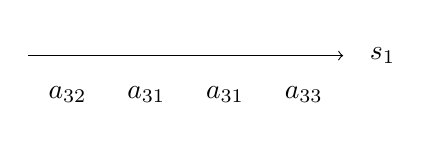
\begin{tikzpicture}
        \node [circle] (a11) at (-1.5,0) {$a_{32}$};
        \node [circle] (a12) at (-0.5,0) {$a_{31}$};
        \node [circle] (a13) at (0.5,0) {$a_{31}$};
        \node [circle] (a14) at (1.5,0) {$a_{33}$};
        \draw [->] (-2,0.5) -- (2,0.5);
        \node [circle] (s1) at (2.5,0.5) {$s_1$};
    \end{tikzpicture}
    \caption{用 \ttt{im\_{}1} 获取数组片段结果图}
    \label{a_section__example_2}
\end{figure}

我接着讲用三元下标 (vector subscript\footnote{\href{https://j3-fortran.org/doc/year/24/24-007.pdf}{标准解释文档}里用的词是 ``subscript triplet'', 可翻译成 ``下标三元组''.}) 来获取数组片段. 三元下标是 \ttt{m1:m2:m3}, 等价于向量下标 \ttt{[(i, i = m1, m2, m3)]}, 请注意这是官规而不是 Ifx 的器规, 并且三元下标两边没有左右中括号 \ttt{[]}. 若省略 \ttt{m1}/\ttt{m2}, 则 \ttt{m1}/\ttt{m2} 是用于获取片段的数组的, 三元下标对应的维度的上界/下界. 若省略 \ttt{:m3}, 则 \ttt{m3} 是 \ttt{1}. 请看下面这个例子.
\begin{lstlisting}
program main
    implicit none
    integer :: i, a(3, 3)
    a = reshape([(i, i = 1, 9)], [3, 3])
    print *, a(::2, 2)
end program main
\end{lstlisting}
这个例子中, 三元下标 \ttt{::2} 对应 \ttt{a} 的第 $1$ 个维度, \ttt{a} 的第 $1$ 个维度的上界和下界分别是 $1$ 和 $3$, 所以 \ttt{::2} 等价于 \ttt{1:3:2}, 亦即等价于 \ttt{[(i, i = 1, 3, 2)]}, 亦即等价于 \ttt{[1, 3]}. 并且数组片段的第 $2$ 个维度被灭掉. 所以这个例子中数组片段的维数为 $1$, 形状为 $[2]$, 如图 \ref{a_section__example_3} 所示.
\begin{figure}[htbp]
    \centering
    \begin{tikzpicture}
        \node [circle] (a11) at (0,0.5) {$a_{12}$};
        \node [circle] (a21) at (0,-0.5) {$a_{32}$};
        \draw [->] (-0.5,1) -- (-0.5,-1);
        \node [circle] (s1) at (-0.5,-1.5) {$s_1$};
    \end{tikzpicture}
    \caption{用三元下标获取数组片段结果图}
    \label{a_section__example_3}
\end{figure}
学 Fortran 的 Matlab 的三元下标用法和 Fortran 相同, 而 C 和学 C 的 Python 的三元下标用法和 Fortran 不相同, 请同学们注意.

同学们如果学数组片段学得晕乎, 请至少掌握使用三元下标 \ttt{m1:m2} 且 \ttt{m1 <= m2} 的情形, 此情形很常用. 若 \ttt{a} 是数组, 且任意 \ttt{m1\_{}i:m2\_{}i}, \ttt{m1\_{}i <= m2\_{}i}, 则 \ttt{a(m1\_{}1:m2\_{}1, ..., m1\_{}n:m2\_{}n)} 代表把 \ttt{a} 的元素中第 \ttt{i} 个下标不在左右闭区间 $[$\ttt{m1\_{}i}$,$ \ttt{m2\_{}i}$]$ 中的元素灭掉得到的数组片段. 请看下面这个例子.
\begin{lstlisting}
program main
    implicit none
    integer :: i, a(3, 3)
    a = reshape([(i, i = 1, 9)], [3, 3])
    print *, a(1:2, 2:3)
end program main
\end{lstlisting}
先将 \ttt{a} 的元素排成表. 第 $1$ 个三元下标是 \ttt{1:2}, 而 $3$ 不在 $[1,2]$ 中, 所以灭掉 \ttt{a} 的元素中第 $1$ 个下标是 $3$ 的元素. 第 $2$ 个三元下标是 \ttt{2:3}, 而 $1$ 不在 $[2,3]$ 中, 所以灭掉 \ttt{a} 的元素中第 $2$ 个下标是 $1$ 的元素. 灭掉元素后如图 \ref{simple_a_step_1} 所示, 没被灭掉的元素合成的就是最后结果.
\begin{figure}[htbp]
    \centering
    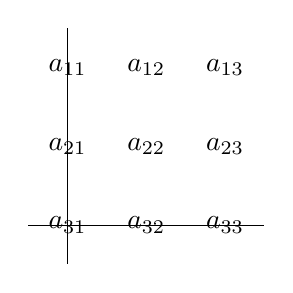
\begin{tikzpicture}
        \node [circle] (a11) at (-1,1) {$a_{11}$};
        \node [circle] (a12) at (0,1) {$a_{12}$};
        \node [circle] (a13) at (1,1) {$a_{13}$};
        \node [circle] (a21) at (-1,0) {$a_{21}$};
        \node [circle] (a22) at (0,0) {$a_{22}$};
        \node [circle] (a23) at (1,0) {$a_{23}$};
        \node [circle] (a31) at (-1,-1) {$a_{31}$};
        \node [circle] (a32) at (0,-1) {$a_{32}$};
        \node [circle] (a33) at (1,-1) {$a_{33}$};
        \draw [-] (-1,1.5) -- (-1,-1.5);
        \draw [-] (-1.5,-1) -- (1.5,-1);
    \end{tikzpicture}
    \caption{用简单三元下标获取数组片段结果图}
    \label{simple_a_step_1}
\end{figure}

本节讲的数组操作, 得到的都是非全数组. 非全数组没有确定的下标, 所以对非全数组取元素/片段将会失败. 例如下面这个程序对数组片段 \ttt{a(:, :)} 再取片段不成.
\begin{lstlisting}
program main
    implicit none
    integer :: i, a(3, 3)
    a = reshape([(i, i = 1, 9)], [3, 3])
    print *, a(:, :)(:, :) ! Invalid!
end program main
\end{lstlisting}

\section{数组赋值}\label{fortran_array_assignment}

给数组 \ttt{\{var\}} 用 \ttt{\{var\} = \{expr\}} 赋值, 情况可分两种, 一种 \ttt{\{expr\}} 是数组, 另一种 \ttt{\{expr\}} 是标量.

如果 \ttt{\{expr\}} 是数组, 那么 \ttt{\{var\}} 和 \ttt{\{expr\}} 形状必须一样. 此时让 \ttt{\{var\}} 和 \ttt{\{expr\}} 一一对应的元素相等. 示例如下, 其中 \ttt{\{expr\}} 是非全数组, 上下界不定, 但元素的一一对应关系和上下界无关, 所以赋值可行.
\begin{lstlisting}
program main
    implicit none
    integer :: i
    real :: a(3, 3)
    a = reshape([(real(i), i = 1, 9)], [3, 3])
    a = -a
    do i = 1, 3
        print *, a(i, :)
    end do
end program main
\end{lstlisting}

如果 \ttt{\{var\}} 是延迟形状数组, 那么 \ttt{\{var\}} 和 \ttt{\{expr\}} 维数必须一样, 此时 \ttt{lbound(\{var\})} 和 \ttt{ubound(\{var\})} 分别是 \ttt{lbound(\{expr\})} 和 \ttt{ubound (\{expr\})}. 示例如下, 其中 \ttt{\{expr\}} 是非全数组, 则 \ttt{lbound(\{var\})} 和 \ttt{ubound(\{var\})} 分别是 $[1,1]$ 和 $[3,3]$.
\begin{lstlisting}
program main
    implicit none
    integer :: i
    real, allocatable :: a(:, :)
    a = reshape([(real(i), i = 1, 9)], [3, 3])
    do i = 1, 3
        print *, a(i, :)
    end do
    print *, lbound(a)
    print *, ubound(a)
    deallocate(a)
end program main
\end{lstlisting}

如果 \ttt{\{expr\}} 是标量, 那么先临时造一个形状与 \ttt{\{var\}} 一样, 而其中元素皆为 \ttt{\{expr\}} 的数组 \ttt{\{expr\_{}\}}, 然后执行 \ttt{\{var\} = \{expr\_{}\}}. 示例如下.
\begin{lstlisting}
program main
    implicit none
    integer :: i
    real :: a(3, 3)
    a = 0.0
    do i = 1, 3
        print *, a(i, :)
    end do
end program main
\end{lstlisting}
如果 \ttt{\{var\}} 是延迟形状数组且形状未定, 那么执行 \ttt{\{var\} = \{expr\}} 将失败. 错误示例如下, 此程序 Ifx 能跑起, 原因应该是 Ifx 在 \ttt{\{var\}} 形状未定的情况下, 会自己认定 \ttt{\{var\}} 的各维度的长度是 $0$.
\begin{lstlisting}
program main
    implicit none
    integer :: i
    real, allocatable :: a(:, :)
    a = 0.0 ! Invalid!
    do i = 1, 3
        print *, a(i, :)
    end do
    print *, lbound(a)
    print *, ubound(a)
    deallocate(a)
end program main
\end{lstlisting}
如果 \ttt{\{var\}} 是延迟形状数组且形状已定, 那么 \ttt{\{var\}} 的各维度的上界和下界虽被重定, 但重定后的各维度的上界和下界和重定前的各维度的上界和下界相同, 相当于上界和下界没被重定, 并且随后执行 \ttt{\{var\} = \{expr\}}. 示例如下.
\begin{lstlisting}
program main
    implicit none
    integer :: i
    real, allocatable :: a(:, :)
    allocate(a(0:2, 0:2))
    a = 0.0
    do i = 1, 3
        print *, a(i, :)
    end do
    print *, lbound(a)
    print *, ubound(a)
    deallocate(a)
end program main
\end{lstlisting}

仿照对整个数组赋值, 我们可以轻松地对数组元素/片段赋值, 示例如下, 示例中数组元素 \ttt{a(3, 1)} 被赋值成 \ttt{0}, 数组片段 \ttt{a(1:2, 2:3)} 对应的元素 \ttt{a(2, 1)}, \ttt{a(2, 2)}, \ttt{a(3, 1)}, \ttt{a(3, 2)} 分别被赋值成 \ttt{1}, \ttt{2}, \ttt{3}, \ttt{4}, 其他元素不变. 
\begin{lstlisting}
program main
    implicit none
    integer :: i, a(3, 3)
    a = reshape([(i, i = 1, 9)], [3, 3])
    a(3, 1) = 0
    a(1:2, 2:3) = reshape([(i, i = 1, 4)], [2, 2])
    do i = 1, 3
        print *, a(i, :)
    end do
end program main
\end{lstlisting}

Fortran 数组赋值是并行 (parallel) 计算, 请看下面的例子.
\begin{lstlisting}
program main
    implicit none
    integer :: i, a(9)
    a = [(i, i = 1, 9)]
    a(2:9) = a(1:8)
    print *, a
end program main
\end{lstlisting}
在上面的例子中, \ttt{a(1)} 赋值给 \ttt{a(2)}, \ttt{a(2)} 赋值给 \ttt{a(3)}, \dots{}, \ttt{a(8)} 赋值给 \ttt{a(9)}, 这些赋值是需要\uline{同时}进行的, 最后 \ttt{a} 是 $[1,1,2,3,4,5,6,7,8]$. 同时进行多个计算就是并行计算, 当然这需要电脑有同时进行多个计算的能力. 如果电脑不行, 比如安安用家里的老破电脑跑上面的例子, 电脑每时每刻总是只能进行一个计算, 此时编译器和电脑会自己想办法操作一波, 模拟同时进行多个计算, 以保证最后干出来的结果和那些能同时进行多个计算的好电脑干出来的结果一样, 这样的计算就是并发 (concurrent) 计算. 又请看下面的例子.
\begin{lstlisting}
program main
    implicit none
    integer :: i, a(9)
    a = [(i, i = 1, 9)]
    do i = 1, 8
        a(i+1) = a(i)
    end do
    print *, a
end program main
\end{lstlisting}
这个例子不一样, \ttt{a(1)} 赋值给 \ttt{a(2)}, 所以 \ttt{a(2)} 变成 \ttt{1}, \ttt{a(2)} 赋值给 \ttt{a(3)}, 所以 \ttt{a(3)} 变成 \ttt{1}, \dots{}, \ttt{a(8)} 赋值给 \ttt{a(9)}, 所以 \ttt{a(9)} 变成 \ttt{1}, 这些赋值是需要\uline{按顺序依次}进行的, 最后 \ttt{a} 是 $[1,1,1,1,1,1,1,1,1]$. 按顺序依次多个计算就是串行 (serial) 计算.

并行计算我们是非常需要的, 因为能省大量时间, 比如我们有一个大小为 $1000\times1000$ 的数组 (这样大的数组实践中并不罕见). 如果我们的电脑, 比如一台超级计算机, 能同时进行 $1\times{10}^6$ 个计算, 程序运行时我们给数组赋值很多次, 总共用时 $1$ 秒. 如果我们的电脑, 比如安安家里的老破电脑, 只能同时进行 $1$ 个计算, 程序运行时我们给数组赋值很多次, 总共用时 $1\times{10}^6$ 秒 $>$ $10$ 天, 用时太多了. Fortran 的语法可以直接区分串行计算和并行计算, 这是 Fortran 的巨大优势 (Python 的 Numpy 已借鉴).

数组赋值还可以用 forall 结构, where 结构和 do concurrent 结构, 其中 forall 结构已被弃用, 加之同学们学完 where 结构和 do concurrent 结构估计已经晕菜了, 安安拒讲 forall 结构. 同学们如果弄不懂 where 结构和 do concurrent 结构可以先不掌握, 因为不用这俩玩意儿同学们也能干活儿, 就是程序跑得可能比较慢, 但其他数组赋值方法同学们必须掌握, 不然期末一定挂科呢.

\subsection{where 结构}\label{where_construct}

实践中我们经常会碰到需要 ``根据数组元素的性质决定对元素的操作'' 的情况. 假如有个数组 \ttt{a}, 我们想让 \ttt{a} 中 \ttt{<= 3} 的元素都加上 \ttt{2}, 让 \ttt{a} 中不 \ttt{<= 3} 且 \ttt{<= 6} 的元素都加上 \ttt{2}, 让 \ttt{a} 中其他元素都加上 \ttt{3}, 我们可以傻乎乎地用双重 do 循环加 if 判断这么写.
\begin{lstlisting}
program main
    implicit none
    integer :: i, j, a(3, 3)
    a = reshape([(i, i = 1, 9)], [3, 3])
    do i = 1, 3
        do j = 1, 3
            if (a(i, j) <= 3) then
                a(i, j) = a(i, j) + 1
            else if (a(i, j) <= 6) then
                a(i, j) = a(i, j) + 2
            else
                a(i, j) = a(i, j) + 3
            end if
        end do
    end do
    do i = 1, 3
        print *, a(i, :)
    end do
end program main
\end{lstlisting}
Fortran 党看这个程序要跳脚, 因为第一这个程序太冗长, 第二这个程序的双重 do 循环里是完全串行计算的. 我们可以使用 where 结构进行掩码数组赋值, 改写上面的程序成下面的程序, 其中 \ttt{tag} 是 where 结构的标签, 可省去, 并且注释标注的行分别都是并行计算的. 相信同学们能总结出 where 结构的用法. 另外 where 结构和 if 结构的语法很像但又有点不一样, 请同学们自己对比, 不要混淆.
\begin{lstlisting}
program main
    implicit none
    integer :: i, a(3, 3)
    a = reshape([(i, i = 1, 9)], [3, 3])
    tag: where (a <= 3)
        a = a + 1 ! Parallel!
    elsewhere (a <= 6)
        a = a + 2 ! Parallel!
    elsewhere
        a = a + 3 ! Parallel!
    end where tag
    do i = 1, 3
        print *, a(i, :)
    end do
end program main
\end{lstlisting}
又假如有个数组 \ttt{a}, 我们想让 \ttt{a(1:2, 2:3)} 中 \ttt{<= 3} 的元素都加上 \ttt{2}, 让 \ttt{a(1:2, 2:3)} 中不 \ttt{<= 3} 且 \ttt{<= 6} 的元素都加上 \ttt{2(1:2, 2:3)}, 让 \ttt{a(1:2, 2:3)} 中其他元素都加上 \ttt{3}, 我们可以这么写.
\begin{lstlisting}
program main
    implicit none
    integer :: i, a(3, 3)
    a = reshape([(i, i = 1, 9)], [3, 3])
    tag: where (a(1:2, 2:3) <= 3)
        a(1:2, 2:3) = a(1:2, 2:3) + 1 ! Parallel!
    elsewhere (a(1:2, 2:3) <= 6)
        a(1:2, 2:3) = a(1:2, 2:3) + 2 ! Parallel!
    elsewhere
        a(1:2, 2:3) = a(1:2, 2:3) + 3 ! Parallel!
    end where tag
    do i = 1, 3
        print *, a(i, :)
    end do
end program main
\end{lstlisting}
又假如有个数组 \ttt{a} 且有个数组 \ttt{b}, 它们形状一样, 我们想当 \ttt{a(i, j) <= 3} 时 \ttt{b(i, j)} 加上 \ttt{1}, 当不 \ttt{a(i, j) <= 3} 且 \ttt{a(i, j) <= 6} 时 \ttt{b(i, j)} 加上 \ttt{2}, 其他情况 \ttt{b(i, j)} 加上 \ttt{3}, 我们可以这么写.
\begin{lstlisting}
program main
    implicit none
    integer :: i, a(3, 3), b(3, 3)
    a = reshape([(i, i = 1, 9)], [3, 3])
    b = reshape([(i, i = 1, 9)], [3, 3])
    tag: where (a <= 3)
        b = b + 1 ! Parallel!
    elsewhere (a <= 6)
        b = b + 2 ! Parallel!
    elsewhere
        b = b + 3 ! Parallel!
    end where tag
    do i = 1, 3
        print *, b(i, :)
    end do
end program main
\end{lstlisting}

看懂上面几个示例的同学会觉得 where 结构真好用, 但请这些同学不要高兴得太早, where 结构乍看着方便, 实则正因如此而有一个 Fortran 没学好的人不可能知道的坑. 要懂得这个坑, 同学们需要先学习 \ref{elemental_procedure} 小节然后倒回头来看这里. 来看下面这个\href{https://j3-fortran.org/doc/year/24/24-007.pdf}{标准解释文档}里给的经典程序.
\begin{lstlisting}
program main
    implicit none
    integer :: i
    real :: a(9)
    a = [(real(i), i = -4, +4)]
    where(a > 0.0)
        ! log is invoked only for positive elements,
        ! because log is elemental.
        a = log(a) 
    end where
    print *, a
    print *, a / sum(a)
    a = [(real(i), i = -4, +4)]
    where(a > 0.0)
        ! log is invoked for ALL elements,
        ! because sum is NOT elemental.
        a = a / sum(log(a)) 
    end where
    print *, a
end program main
\end{lstlisting}
在这个程序中, \ttt{a = log(a)} 里的 \ttt{log} 是逐元函数, 所以 \ttt{log(a)} 里的 \ttt{a} 代表的是 \ttt{a} 的元素 \ttt{> 0.0} 的部分, 所以这个程序中的 \ttt{a = log(a)} 相当于 \ttt{a(6:9) = log(a(6:9))}. 而 \ttt{a = a / sum(log(a))} 里的 \ttt{sum} \uline{不是}逐元函数, \ttt{sum(log(a))} 里的 \ttt{a} 出现在非逐元函数的 \ttt{sum} 后跟的括号 \ttt{()} 里, 这时请注意, \ttt{sum(log(a))} 里的 \ttt{a} 代表的不是 \ttt{a} 的元素 \ttt{> 0.0} 的部分, 而是 \ttt{a} \uline{整个数组}, 即便 \ttt{log} 是逐元函数也不影响这点, 所以这个程序中的 \ttt{a = a / sum(log(a))} 相当于 \ttt{a(6:9) = a(6:9) / sum(log(a(:)))}.

\subsection[do concurrent\\结构]{do concurrent 结构}

有些程序不好用 where 结构改写, 比如下面的程序.
\begin{lstlisting}
program main
    implicit none
    integer :: i, j, a(9), b(9)
    a = [(i, i = 1, 9)]
    b = [(j, j = 1, 9)]
    do i = 1, 3, 1
        do j = 7, 9, 1
            if ((a(i) > 1) .and. (b(j) < 9)) then
                b(i) = -j
                a(j) = -i
            end if
        end do
    end do
    print *, a
    print *, b
end program main
\end{lstlisting}
我们可以使用同样是并行计算的 do concurrent 结构\footnote{\href{https://j3-fortran.org/doc/year/24/24-007.pdf}{标准解释文档}把 do concurrent 结构划成 do 结构中的一种, 但一般还是把 do concurrent 结构单看成一种结构.}来改写上面的程序成下面的程序, 其中 \ttt{tag} 是 do concurrent 结构的标签, 可省去, 两个 \ttt{:1} 因为是 \ttt{:\{m3\}} 所以也可省去, 但 \ttt{\{m1\}} 和 \ttt{\{m2\}} \uline{不可}省去. 相信同学们能总结出 do concurrent 结构的用法. 另外 do concurrent 结构和 do 结构, where 结构和数组三元下标的语法很像但又有点不一样, 请同学们自己对比, 不要混淆.
\begin{lstlisting}
program main
    implicit none
    integer :: i, j, a(9), b(9)
    a = [(i, i = 1, 9)]
    b = [(j, j = 1, 9)]
    tag: do concurrent (i = 1:3:1, j = 7:9:1, &
                        (a(i) > 1) .and. (b(j) < 9))
        b(i) = -j
        a(j) = -i
    end do tag
    print *, a
    print *, b
end program main
\end{lstlisting}

\section{数组运算}\label{fortran_array_operation}

如果一个代表运算 $\text{OP}$ 的一元运算符 \ttt{\{op\}} 右跟 \ttt{\{q\}}, 且 \ttt{\{q\}} 是数组, 那么结果的形状与 \ttt{\{q\}} 一样, 且任意 \ttt{\{q\}} 的元素 $q_{s_1\dots s_n}$, \ttt{\{op\}\{q\}} 中与 $q_{s_1\dots s_n}$ 对应的元素为 $\text{OP}\,q_{s_1\dots s_n}$. 示例如下.
\begin{lstlisting}
program main
    implicit none
    integer :: i
    real :: a(3, 3)
    a = reshape([(real(i), i = 1, 9)], [3, 3])
    a = -a
    do i = 1, 3
        print *, a(i, :)
    end do
end program main
\end{lstlisting}

如果一个代表运算 $\text{OP}$ 的二元运算符 \ttt{\{op\}} 左右分别跟 \ttt{\{q1\}} 和 \ttt{\{q2\}}, 且 \ttt{\{q1\}} 和 \ttt{\{q2\}} 是形状相同的数组, 那么结果的形状也相同, 且任意 \ttt{\{q1\}} 和 \ttt{\{q2\}} 的元素 ${q_1}_{ s_1\dots s_n }$ 和 ${q_2}_{ s_1\dots s_n }$, \ttt{\{q1\}\{op\}\{q2\}} 中与 ${q_1}_{ s_1\dots s_n }$ 和 ${q_2}_{ s_1\dots s_n }$ 对应的元素为 ${q_1}_{ s_1\dots s_n }\,\text{OP}\,{q_2}_{ s_1\dots s_n }$. 示例如下.
\begin{lstlisting}
program main
    implicit none
    integer :: i
    real :: a(3, 3)
    a = reshape([(real(i), i = 1, 9)], [3, 3])
    a = a * a
    do i = 1, 3
        print *, a(i, :)
    end do
end program main
\end{lstlisting}
如果一个代表运算 $\text{OP}$ 的二元运算符 \ttt{\{op\}} 左右分别跟 \ttt{\{q1\}} 和 \ttt{\{q2\}}, 且 \ttt{\{q1\}} 和 \ttt{\{q2\}} 是形状不同的数组, 那么运算将失败. 错误示例如下.
\begin{lstlisting}
program main
    implicit none
    integer :: i
    real :: a(3, 3)
    a = reshape([(real(i), i = 1, 9)], [3, 3])
    a = a(3, :) * a(3:3, :) ! Invalid!
    do i = 1, 3
        print *, a(i, :)
    end do
end program main
\end{lstlisting}
如果一个代表运算 $\text{OP}$ 的二元运算符 \ttt{\{op\}} 左右分别跟 \ttt{\{q1\}} 和 \ttt{\{q2\}}, 且 \ttt{\{q1\}} 和 \ttt{\{q2\}} 一个是标量一个是数组, 那么先临时把 \ttt{\{q1\}} 和 \ttt{\{q2\}} 中是标量的那个替换成一数组, 此数组形状与 \ttt{\{q1\}} 和 \ttt{\{q2\}} 中是数组的那个一样, 且此数组中元素皆为 \ttt{\{q1\}} 和 \ttt{\{q2\}} 中是标量的那个, 然后按 \ttt{\{q1\}} 和 \ttt{\{q2\}} 是形状相同的数组时的方法进行运算. 示例如下.
\begin{lstlisting}
program main
    implicit none
    integer :: i
    real :: a(3, 3)
    a = reshape([(real(i), i = 1, 9)], [3, 3])
    a = a(3, 3) * a
    do i = 1, 3
        print *, a(i, :)
    end do
end program main
\end{lstlisting}

本节讲的数组运算, 得到的都是非全数组. 所以下面这个程序不成.
\begin{lstlisting}
program main
    implicit none
    integer :: i
    real :: a(3, 3)
    a = reshape([(real(i), i = 1, 9)], [3, 3])
    print *, (-a)(3, 3) ! Invalid!
end program main
\end{lstlisting}
但下面这个程序成, 因为数组取元素/片段优先于数组运算, 所以 \ttt{-a(3, 3)} 实际上代表 \ttt{-(a(3, 3))}, 没有问题.
\begin{lstlisting}
program main
    implicit none
    integer :: i
    real :: a(3, 3)
    a = reshape([(real(i), i = 1, 9)], [3, 3])
    print *, -a(3, 3)
end program main
\end{lstlisting}
